\documentclass{article}
\usepackage{listings}
\usepackage{caption}
\usepackage{subcaption}
\usepackage{booktabs}
\usepackage[utf8]{inputenc}
\usepackage{amsmath}
\usepackage{amsthm}
\usepackage{amssymb}
\usepackage{pgfplots}
\usepackage{float}
\usepackage{pstricks, pst-plot, pst-node}
\usepackage{xcolor}
\usepackage{braket}
\usepackage[colorinlistoftodos]{todonotes}
\usepackage[noend]{algpseudocode}
\usepackage{hyperref}
\usepackage{algpseudocode,algorithm,algorithmicx}

\usepackage[T1]{fontenc}
\usepackage{graphicx}
\usepackage{xcolor}
\usepackage{tgtermes}

\usepackage{amsmath,amssymb,amsthm,textcomp}
\usepackage{enumerate}
\usepackage{multicol}
\usepackage{titling}

\usepackage{graphicx}
\usepackage{epstopdf}

\epstopdfDeclareGraphicsRule{.gif}{png}{.png}{convert gif:#1 png:\OutputFile}
\AppendGraphicsExtensions{.gif}


\usepackage{tikz}

\usepackage[italian]{babel}

\title{Crittografia su curve ellittiche}
\author{Gaspare Ferraro}
\date{24 Giugno 2017}

% Definition of \maketitle
\makeatletter         
\def\@maketitle{
	\raggedright
	\begin{center}
		{\Huge \bfseries \@title }\\[4ex]
		{\Large  \@author}\\[4ex] 
		\@date\\[8ex]
		
\includegraphics[width = 60mm]{logo.png}
\end{center}}
\makeatother


\begin{document}
	
	\maketitle
	\thispagestyle{empty}
	
	\clearpage
	
	\tableofcontents
	
	\clearpage
	
	\section{Il problema della sicurezza}
	
	Con l'avanzare del progresso tecnologico, la diffusione della banda larga e un intenso utilizzo dell'informatica
	nella vita quotidiana, i temi della privacy e sicurezza acquistano maggiore importanza.\\
	
	Per questo motivo necessitiamo di sistemi crittografici sempre più avanzati per garantire affidabilità 
	nelle comunicazioni, un esempio è la crittografia su curve ellittiche, descritta in questa relazione, 
	che rappresenta un'ottima alternativa al più noto metodo RSA
	\footnote{Algoritmo di crittografia asimmetrica, dalle iniziali dei suoi inventori (Rivest-Shamir-Adleman), basato sul problema della fattorizzazione.   } 
	sotto molti aspetti.\\
	
	Le curve ellittiche, particolari curve algebriche con le quali è possibile definire un sistema crittografico,
	sono ampiamente usate in famosi contesti come ad esempio il browser Google Chrome
	\footnote{ECDSA for WebRTC: Better Security, Better Privacy and Better Performance: \url{https://developers.google.com/web/updates/2016/06/webrtc-ecdsa}} e la criptovaluta Bitcoin.\\
	
	I primi capitoli saranno dedicati ad una presentazione teorica delle curve ellittiche in matematica, 
	verranno poi illustrati gli utilizzi pratici delle curve ellittiche in crittografia, 
	mentre nell'ultimo capitolo si analizzeranno gli algoritmi implementati e confrontati 
	con il metodo RSA dai punti di vista delle prestazioni e della sicurezza.\\
	
	In appendice è presente la libreria scritta in linguaggio Java che implementa, a scopo didattico, gli algoritmi che verranno successivamente presentati.
	
	\clearpage
	%%%%%%%%%%%%%%%%%%%%%%%%%%%%%%%%%%%%%%%%%%%%%%%%%%%%%%%%%%%%%%%%%%%%%%%%%%%%%%%%%%%%%%%%%%%%%%%
	%%%%%%%%%%%%%%%%%%%%%%%%%%%%%%%%%%%%%%%%%%%%%%%%%%%%%%%%%%%%%%%%%%%%%%%%%%%%%%%%%%%%%%%%%%%%%%%
	
	\section{Curve Ellittiche}
	
	\subsection{Definizioni preliminari}
	
	Per meglio comprendere la definizione di curva ellittica è necessario prima introdurre altre due definizioni.
	
	\newtheorem{defn}{Definizione}
	\newtheorem{teo}{Teorema}
	\begin{defn}[Campo]
		Un campo è una struttura algebrica composta da un insieme non vuoto $\mathbb{K}$ e da due operazioni binarie interne, chiamate $addizione$ e $moltiplicazione$, per le quali valgano le proprietà associativa e commutativa e l'esistenza dell'elemento neutro e dell'inverso di ciascun elemento dell'insieme (tranne al più l'elemento neutro della moltiplicazione).
	\end{defn}
	
	\begin{defn}[Caratteristica di un campo]
		La caratteristica di un campo $\mathbb{K}$ è il più piccolo numero naturale $n$ tale che, sommando $n$ volte l'elemento neutro della moltiplicazione (indicato con il numero $1$), si ottenga l'elemento neutro dell'addizione (indicato con il numero $0$).
		
		\begin{equation}
		\underbrace{1+1+...+1+1}_\text{n volte} = 0
		\end{equation}
		
		Se tale numero $n$ non esiste, la caratteristica del campo è $0$ per definizione.\\
	\end{defn}
	
	Diamo ora la definizione di curva ellittica:
	
	\begin{defn}[Curva ellittica]
		Una curva ellittica $E$ su un campo $\mathbb{K}$ è l'insieme dei punti $(x,y) \in \mathbb{K}^{2}$ che soddisfano l'equazione:
		
		\begin{equation}
		y^{2} + axy + by = x^{3} + cx^{2} + dx + e
		\end{equation}
		
		con $a, b, c, d, e \in \mathbb{K}$.\\
		A questo insieme aggiugiamo un punto $O$ chiamato "punto all'infinito".\\
	\end{defn}
	
	Se la caratteristica del campo $\mathbb{K}$ è diversa da 2 e da 3 è possibile riscrivere l'equazione che definisce la curva ellittica in una forma più compatta (detta forma normale di Weierstrass):
	
	\begin{equation}
	y^{2} = x^{3} + ax + b
	\end{equation}
	
	La cosa che rende interessanti le curve ellittiche in crittografia è la possibilità di definire una struttura algebrica di gruppo abeliano additivo.
	Tale struttura è caratterizzata dalla legge di gruppo, ovvero un'operazione binaria interna chiamata somma (tra punti di una curva ellittica), che gode delle proprietà di associatività e commutatività, con elemento neutro ed esistenza dell'inverso per ogni punto.
	
	\subsection{Curve ellittiche su $\mathbb{R}$}
	
	Analizziamo inizialmente le curve ellittiche definite sul campo $\mathbb{R}$, di più facile comprensione, ricordando dalla definizione 1 che il campo $\mathbb{R}$ ha caratteristica 0.
	
	I punti di una curva ellittica su $\mathbb{R}$, di parametri $a, b \in \mathbb{R}$, sono i punti dell'insieme $E(a,b)$ definito come:
	
	\begin{equation}
	E(a,b) = \set{ (x,y) \in \mathbb{R}^2 | y^{2} = x^{3} + ax + b }
	\end{equation}
	
	Con l'assunzione che $4a^{3} + 27b^{2} \neq 0$, 
	condizione necessaria per la non singolarità della curva, ovvero l'assenza di punti non singolari dove non è definita una tangente.
	
	\begin{figure}[H]
		\centering
		\begin{subfigure}{.5\textwidth}
			\centering
			
			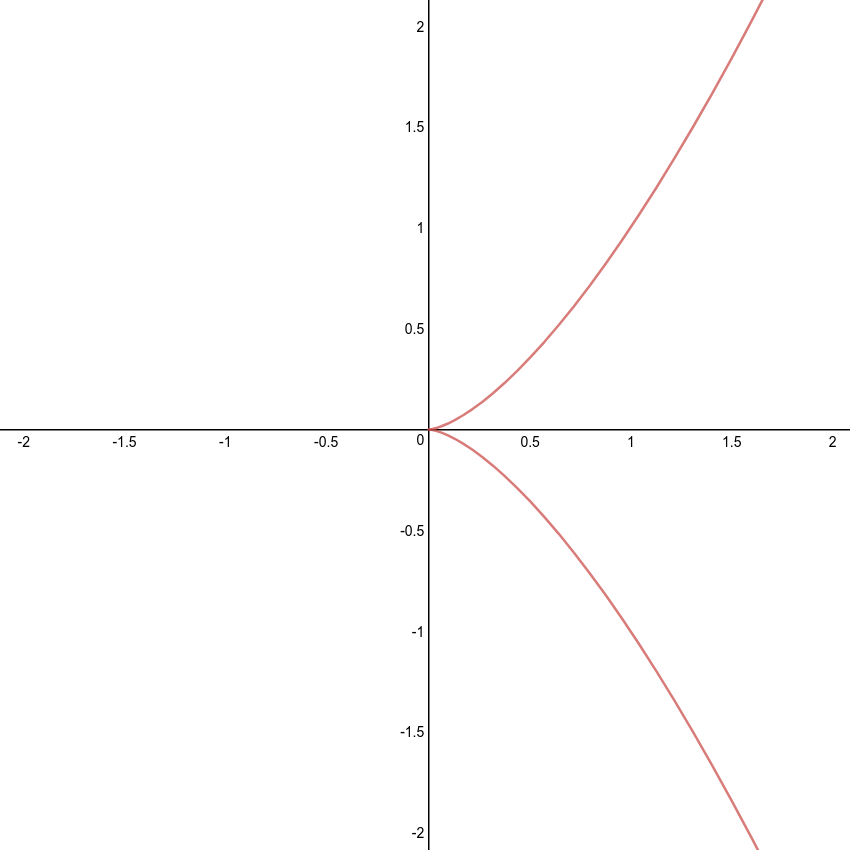
\includegraphics[width=5cm, height=5cm]{img/img1}
			
			
			\caption{Curva ellittica singolare $y^{2} = x^{3}$}
			\label{fig:fig1}
		\end{subfigure}%
		\begin{subfigure}{.5\textwidth}
			\centering
			
			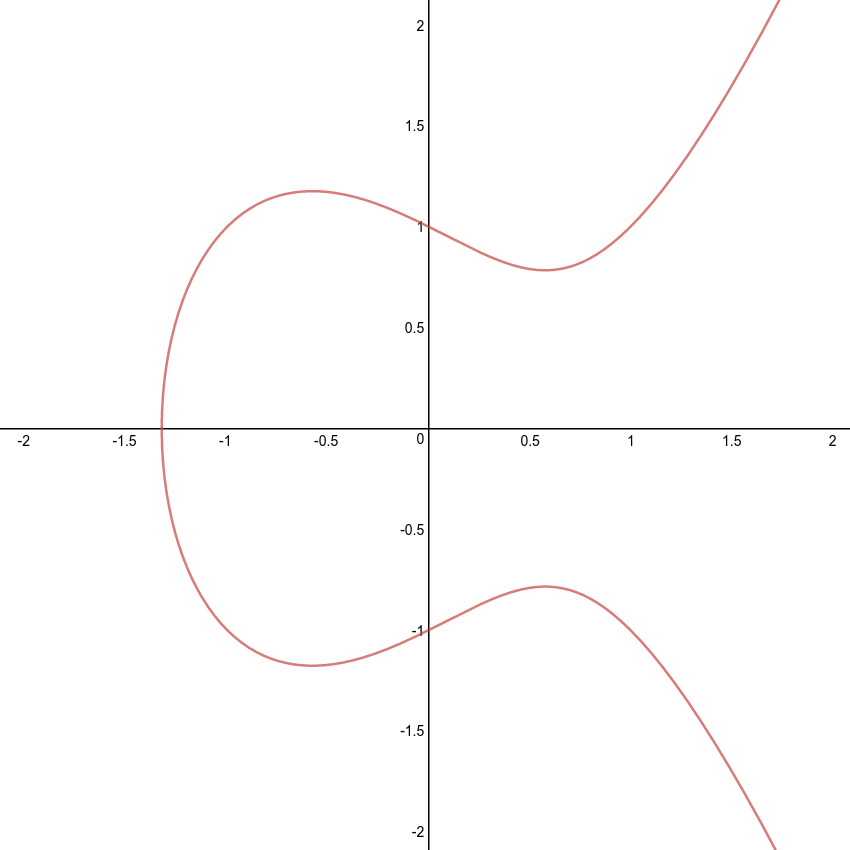
\includegraphics[width=5cm, height=5cm]{img/img2}
			
			\caption{Curva ellittica non singolare $y^{2} = x^{3} - x + 1$}
			\label{fig:fig2}
		\end{subfigure}
		
		%\caption{Esempi di curve ellittiche}
		
	\end{figure}
	
	Possiamo ora dare una spiegazione intuitiva della somma in modo geometrico: considerati due punti $P, Q \in E(a,b)$ con $Q \neq P$ e $Q \neq O$, la somma $P + Q = R$ si ottiene tracciando una retta passante per i punti $P$ e $Q$, che interseca la curva in un punto $R'$. Il punto $R$ cercato è quindi il punto simmetrico a $R'$ rispetto all'asse delle ascisse, un esempio di tale procedimento:
	
	\begin{figure}[H]
		\centering
		
		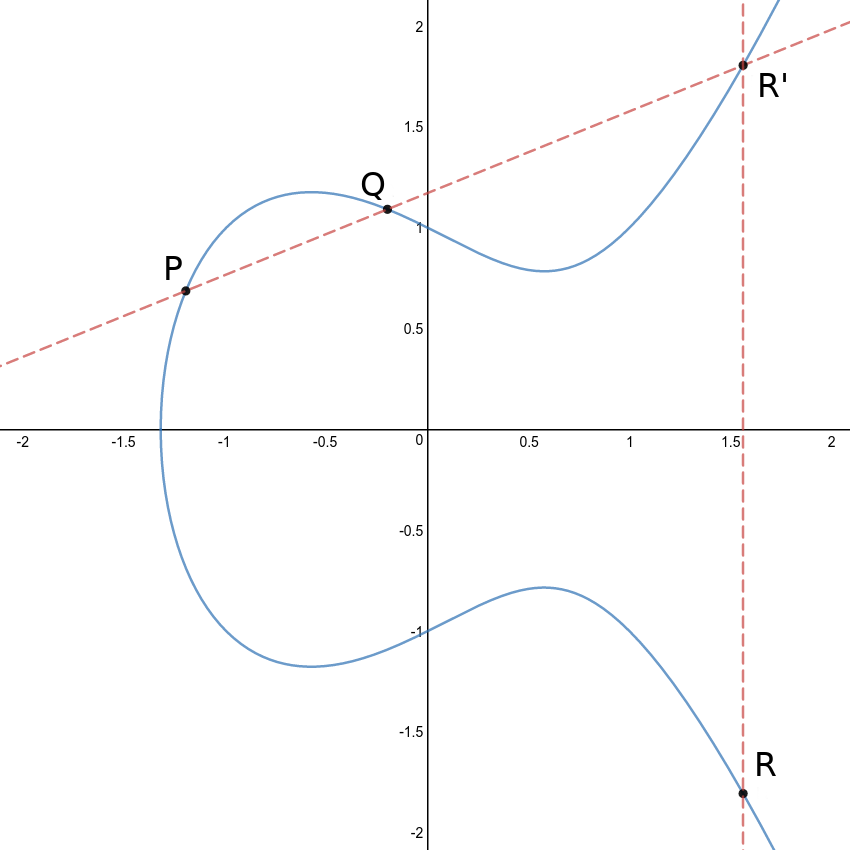
\includegraphics[width=5.5cm, height=5.5cm]{img/img3}
		
		\caption{Somma dei punti $P$ e $Q$}
		\label{fig:fig3}
	\end{figure}%
	
	Nel caso $Q = P$, la somma $P+P = 2P$ (raddoppio del punto $P$) è, invece, ottenuta tracciando la retta tangente passante per $P$ (che esiste sempre, poichè la curva è non singolare per assunzione), analogalmente alla somma generale tale retta interseca la curva in un punto $R'$ del quale si prende il punto simmetrico $R$ rispetto all'asse delle ascisse. Un esempio in figura:\\
	
	\begin{figure}[H]
		\centering
		
		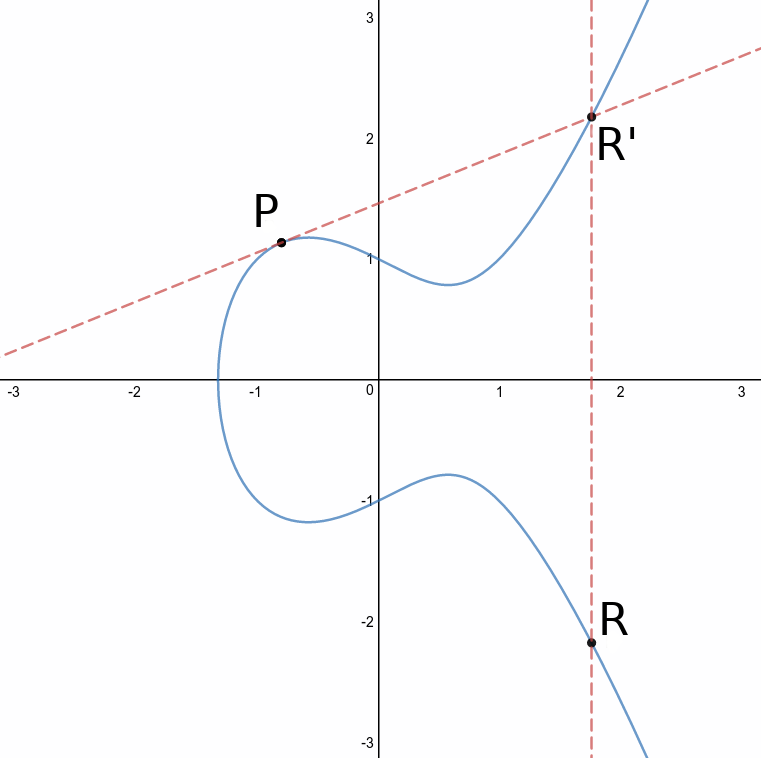
\includegraphics[width=5.5cm, height=5.5cm]{img/img4}
		
		\caption{Raddoppio del punto $P$}
		\label{fig:fig4}
	\end{figure}%
	
	
	Infine, nel caso in cui $Q = O$ (somma del punto P con il punto $O$), la retta tracciata è la verticale passante per $P'$ che è il simmetrico $P$ rispetto alle ascisse, il quale punto simmetrico è nuovamente $P$ stesso.\\
	
	\begin{figure}[H]
		\centering
		
		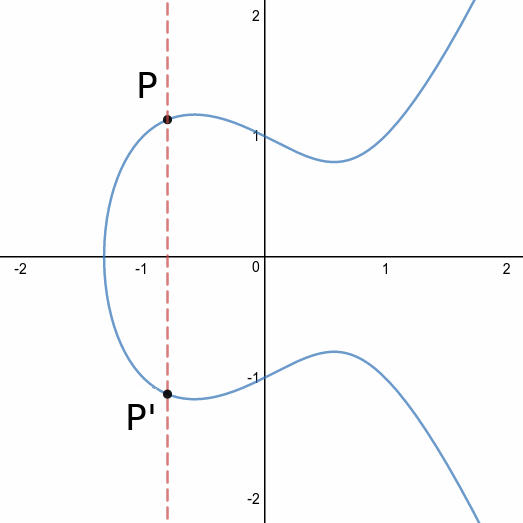
\includegraphics[width=5.5cm, height=5.5cm]{img/img5}
		
		\caption{Raddoppio del punto $P$}
		\label{fig:fig5}
	\end{figure}%
	
	Più formalmente per la somma valgono le seguenti proprietà:
	
	\begin{enumerate}
		\item \textbf{Chiusura}: $\forall P, Q \in E(a,b)$, $P+Q \in E(a,b)$
		
		\item \textbf{Identità}: $\forall P \in E(a,b)$, $P + O = P$
		
		\item \textbf{Opposto}: Sia $P = (x,y) \in E(a,b)$ il suo opposto $-P \in E(a,b)$ è il punto di coordinate $(x, -y)$
		
		\item \textbf{Somma}: Siano $P = (x_{1}, y_{1}), Q = (x_{2}, y_{2}) \in E(a,b)$ con $P \neq Q$ 
		\\ allora $P + Q = R$ con $R = (x_{3}, y_{3}) \in E(a,b)$ dove:
		
		\begin{equation}
		\begin{aligned}
		x_{3} & = \Big (\frac{y_{2} - y_{1}}{x_{2} - x_{1}} \Big )^{2} - x_{1} - x_{2}   \\
		y_{3} & = \Big (\frac{y_{2} - y_{1}}{x_{2} - x_{1}} \Big )(x_{1} - x_{3})-y_{1} 
		\end{aligned}
		\end{equation}
		
		\item \textbf{Raddoppio}: Sia $P = (x_{1},y_{1}) \in E(a,b)$ con $P \neq -P$ \\
		\\allora $P + P = R$ con $R = (x_{2}, y_{2}) \in E(a,b)$ dove:
		
		\begin{equation}
		\begin{aligned}
		x_{2} & = \Big (\frac{3x_{1}^{2}+a}{2y_{1}} \Big )^{2} - 2x_{1}  \\          
		y_{2} & = \Big (\frac{3x_{1}^{2}+a}{2y_{1}} \Big ) (x_{1}-x_{2})-y_{1} 
		\end{aligned}
		\end{equation}
		
		\item \textbf{Associatività}: $\forall P, Q, R \in E(a,b), P+(Q+R) = (P+Q)+R$
		
		\item \textbf{Commutatività}: $\forall P, Q \in E(a,b), P+Q = Q+P$
		
	\end{enumerate}
	
	\subsection{Curve ellittiche su campi finiti}
	
	Più importanti in ambito crittografico ma meno intuitive, sono le curve ellittiche definite sui campi finiti.
	
	\begin{defn}[Campo finito]
		Un campo finito, detto anche campo di Galois, è un campo con un numero finito di elementi.
	\end{defn}
	
	In particolare ogni campo finito ha $p^{n}$ elementi, con $p$ primo e $n$ naturale e, a meno di isomorfismo,
	esiste unico campo finito con $p^{n}$ elementi, che indicheremo con $\mathbb{F}_{p^{n}}$ o $GF(p^{n})$ (dall'inglese Galois Field). \\
	
	Un campo finito $\mathbb{F}_{p^{n}}$ ha caratteristica uguale a $p$, 
	senza perdita di generalità consideriamo solo il caso in cui $p > 3$ che ci permette di scrivere l'equazione
	generale nella forma normale di Weierstrass. \\
	
	\clearpage
	
	Una curva ellittica su un campo finito è quindi l'insieme dei punti definito come:
	
	\begin{equation}
	E_{p^{n}}(a,b) = \set{ (x,y) \in \mathbb{F}_{p^{n}}^{2} | y^{2} = x^{3} + ax + b } \cup \set{O}
	\end{equation}
	
	Per semplicità di operazioni consideriamo le curve con $n=1$, chiamate curve prime, in quanto esiste un isomorfismo $\mathbb{F}_{p} \cong \mathbb{Z}_{p}$.
	In questo campo le operazioni sono quelle dell'algebra modulare, 
	le curva prime sono definite quindi come:
	
	\begin{equation}
	E_{p}(a,b) = \set{ (x,y) \in \mathbb{Z}_{p}^{2} | y^{2} = x^{3} + ax + b \mod p } \cup \set{O}
	\end{equation}
	
	Possiamo notare come le formule definite precedentemente per il campo reale valgano anche 
	per le curve sui campi finiti, ovviamente considerando le operazioni sui relativi campi.\\
	
	I grafici di tali insiemi non sono più delle curve continue, come visto precedentemente,
	ma un insieme finito di punti che soddisfano la definizione, un esempio pratico:
	
	\begin{figure}[H]
		\centering
		
		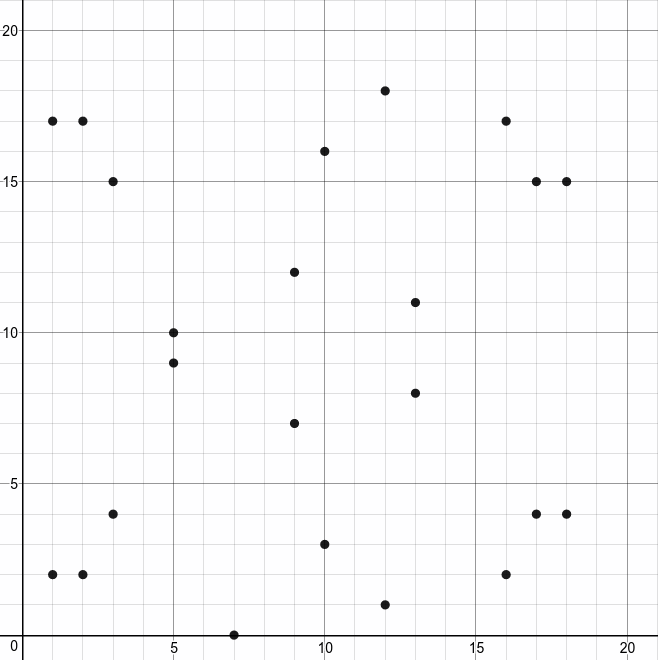
\includegraphics[width=6cm, height=6cm]{img/img6}
		
		\caption{Curva $E_{19}(-7,10)$}
		\label{fig:fig6}
	\end{figure}%
	
	Oltre alle curve prime, nella crittografia su curve ellittiche, si utilizzano inoltre le cosiddette
	curve binarie, definite sul campo $\mathbb{F}_{2^{m}}$, i cui elementi possono essere visti
	come tutti gli interi a $m$ cifre binarie.
	Avendo $\mathbb{F}_{2^{m}}$ caratteristica $2$,
	non è possibile esprimerla con la forma normale di Weierstrass; la curva è quindi definita come:
	
	\begin{equation}
	E_{2^{m}}(a,b) = \set{ (x,y) \in \mathbb{F}_{2^{m}}^{2} | y^{2} + xy = x^{3} + ax^{2} + b }
	\end{equation}
	
	Le curve binarie si prestano ad una migliore implementazione su sistemi hardware, 
	in quanto le operazioni binarie sono facilmente rappresentabili con l'utilizzo di porte logiche
	mentre al contrario, le curve prime, si prestano ad una migliore implementazione su sistemi software.
	Dal punto di vista teorico tutte le operazioni e algoritmi successivamente descritti si applicano 
	indistintamente ad entrambi i tipi di curve.\\
	
	Dalla teoria dell'algebra modulare sappiamo che non sempre esiste la radice quadrata di un numero,
	in generale in $\mathbb{Z}_{p}$ esattamente $(p-1)/2$ elementi sono residui quadratici.
	Ricordando che le curve sono definite per $y^{2}$ e che non tutti i valori di $x$ danno luogo
	ad un residuo quadratico oppure che valori distinti di $x$ possono generare lo stesso residuo quadratico,
	notiamo che alcuni punti delle curve non possono essere definiti.\\
	
	Un parametro importante, basato su questi fatti, che useremo in seguito è l'ordine di una curva.
	
	\begin{defn}[Ordine di una curva ellittica] 
		L'ordine $N$ di una curva ellittica $E_{p^{n}}(a,b)$ è la cardinalità dell'insieme, ovvero il numero dei punti che la compongono.
	\end{defn}
	
	Una curva prima $E_{p}(a,b)$ può evidentemente avere un massimo di $2p+1$ punti: 
	tutte le $p$ coppie di punti $(x, \pm y)$ che soddisfano $y^{2} = x^{3} + ax + b$ e il punto all'infinito.\\
	
	Una stima più accurata sul limite superiore dell'ordine di una curva è data dal seguente teorema:
	
	\begin{teo}[Hasse] 
		L'ordine $N$ di una curva ellittica $E_{p^{n}}(a,b)$ verifica la disuguaglianza $| N - (p^{n} +1) | \leq 2\sqrt{p^{n}}$
	\end{teo}
	
	Mentre non è nota nessuna limitazione inferiore non banale.
	
	\clearpage
	%%%%%%%%%%%%%%%%%%%%%%%%%%%%%%%%%%%%%%%%%%%%%%%%%%%%%%%%%%%%%%%%%%%%%%%%%%%%%%%%%%%%%%%%%%%%%%%
	%%%%%%%%%%%%%%%%%%%%%%%%%%%%%%%%%%%%%%%%%%%%%%%%%%%%%%%%%%%%%%%%%%%%%%%%%%%%%%%%%%%%%%%%%%%%%%%
	
	\section{Il problema del logaritmo discreto}
	
	Per definire un sistema crittografico sulle curve ellittiche, è necessario prima di tutto trovare 
	una funzione one-way trap-door che ne garantisca la sicurezza, ricordiamo che una funzione one-way
	trap-door è una funzione facile da calcolare ma molto difficile da invertire 
	se non si è a conoscenza di particolari informazioni.\\
	
	Nel metodo RSA la funzione one-way trap-door è la fattorizzazione: dati due numeri primi $p$ e $q$, calcolare 
	il loro prodotto $n = pq$ è facile, mentre trovare i due fattori primi conoscendo solo $n$ 
	è un'operazione molto complessa per la quale non si conoscono algoritmi efficienti, 
	conoscendo invece uno dei due fattori ricavare il secondo è banale.\\
	
	In modo analogo all'algebra modulare è possibile dare una definizione di logaritmo discreto per le curve ellittiche
	considerando l'operazione di prodotto scalare:
	
	\begin{defn}[Logaritmo discreto per curve ellittiche]
		Dati due punti di una curva ellittica $P$ e $Q$ chiamiamo, dove è definito, l'intero $k$ per cui $Q = kP$,
		logaritmo in base $P$ del punto $Q$.
	\end{defn}
	
	Notiamo che è possibile calcolare il prodotto $kP$ in modo efficiente utilizzando, invece che $\Theta(k)$ somme, solamente $\Theta(log_{2}k)$ operazioni di raddoppio e $O(log_{2}k)$ somme grazie all'algoritmo dei raddoppi successivi:
	
	\newcommand*\DNA{\textsc{dna}}
	
	\newcommand*\Let[2]{\State #1 $\gets$ #2}
	\algrenewcommand\algorithmicrequire{\textbf{Input:}}
	\algrenewcommand\algorithmicensure{\textbf{Output:}}
	
	
	\makeatletter
	\renewcommand*{\ALG@name}{Algoritmo}
	\makeatother
		
	\begin{algorithm}[H]
		\caption{Calcolo efficiente del prodotto $Q = kP$}
		\begin{algorithmic}[1]
			\Require{intero $k$, punto $P$}
			\Ensure{punto $Q$}
			\Statex
			\Function{fastMult}{$k, P$}
			\Let{$Q$}{$P$}
			\Let{$k$}{$k-1$}
			\While{$k > 0 $}
			\If{$k \mod 2 = 1$}
			\Let{$Q$}{$Q + P$}
			\EndIf
			\Let{$k$}{$k / 2$}
			\Let{$P$}{$2P$}
			\EndWhile
			\State \Return{$Q$}
			\EndFunction
		\end{algorithmic}
	\end{algorithm}
	
	
	Contrariamente al prodotto, l'operazione inversa che consiste nel trovare l'intero $k$ conoscendo i punti $P$ e $Q$, conosciuta come problema del logaritmo discreto per curve ellittiche (ECDLP), non ha algoritmi efficienti noti per risolverlo.\\
	
	Definiamo infine un altro parametro importante in crittografia: l'ordine $n$ di punto $P$ (da non confondere con l'ordine $N$ della curva):
	
	\begin{defn}{Ordine di un punti}
		L'ordine di punto $P$ è il più piccolo intero positivo $n$ tale che $nP = O$ (ovviamente $n \leq N-1$, con $N$ l'ordine della curva).
	\end{defn}
	
	\subsection{Attacchi al problema}
	
	I possibili attacchi noti al problema si possono dividere in due categorie:
	gli algoritmi general-purpose e	quelli special-purpose che sfruttano particolari assunzioni per attaccare determinate classi di curve.\\
	
	Il metodo più famoso è quello chiamato metodo $\rho$ di Pollard, general-purpose, che sfrutta il paradosso dei compleanni per trovare, in $O(\sqrt{N})$ con una probabilità del $50\%$,
	quattro interi $n_{1}$, $n_{2}$, $n_{3}$, $n_{4}$ tali che $n_{1}P + n_{2}Q = n_{3}P + n_{4}Q$.\\ 
	In questo modo sia ha che $k = (n_{1} - n_{3}) / (n_{2} - n_{4}) \mod n$, con $n$ ordine del punto $P$.\\
	
	Altri metodi più complessi special-purpose sono applicabili alle cosiddette curve anomale, 
	con lo scopo di trovare particolari isomorfismi che rendono più facili le operazioni.
	
	\subsection{Scelta della curva}
	
	Gli attacchi noti e altri teoremi matematici sulle curve ellittiche
	ci forniscono fortunatamente alcuni degli accorgimenti \cite{Sec2} nella scelta
	di curve $E_{q}(a,b)$ e dell'utilizzo di particolari punti $P$ di ordine $N$,
	come ad esempio: 
	
	\begin{itemize}
		\item q possibilmente numero primo di Merseinne (ovvero esprimibile nella forma $2^{p}-1$ per qualche primo $p$).
		\item Uso del coefficiente $a = -3$, per ragioni di efficienza, secondo lo standard IEEE P1363 \cite{P1363}.
		\item Il fattore più grande di $N$ deve essere diverso da $q$.
		\item Il numero $N$ deve avere un fattore $r$ tale che un numero di operazioni pari a $\sqrt{r}$ risulti intrattabile.
	\end{itemize}
	
	Per facilitare la scelta, l'agenzia governativa statunitense NIST \footnote{National Institute of Standards and Technology},
	ha pubblicato nel 1999 un documento \cite{NIST} contenente una lista di curve e punti standard da usare,
	privi di difetti dagli attacchi noti. 
	
	
	\clearpage
	%%%%%%%%%%%%%%%%%%%%%%%%%%%%%%%%%%%%%%%%%%%%%%%%%%%%%%%%%%%%%%%%%%%%%%%%%%%%%%%%%%%%%%%%%%%%%%%
	%%%%%%%%%%%%%%%%%%%%%%%%%%%%%%%%%%%%%%%%%%%%%%%%%%%%%%%%%%%%%%%%%%%%%%%%%%%%%%%%%%%%%%%%%%%%%%%
	
	\section{Crittografia su curve ellittiche}
	
	Andiamo ora ad illustrare i più famosi algoritmi di crittografia basati
	sulle curve ellittiche, assumendo che i messaggi da criptare siano dei numeri interi
	che rappresentano, in qualche codifica, le informazioni da trasmettere.
	
	
	\subsection{Codifica dei messaggi}
	
	Siccome tutte le operazioni viste finora, sulle curve ellittiche, coinvolgono solo punti
	appartenenti alle curve e non numeri interi, occorre prima trasformare il messaggio $m$ 
	in un punto $P$ della curva prima o binaria. Purtroppo non sono noti algoritmi deterministici polinomiali, tuttavia esistono degli algoritmi randomizzati molto efficienti che hanno una probabilità bassa di non trovare punti sulla curva. Uno dei più famosi che illustriamo è l'algoritmo di Koblitz.
	
	\begin{algorithm}[H]
		\caption{Codifica di un messaggio $m$ in un punto $P$ della curva $E_{p}(a,b)$}
		\begin{algorithmic}[1]
			\Require{$m$ messaggio; $p, a, b$ parametri della curva prima; $h$ intero positivo fissato tale che $(m+1)h < p$ }
			\Ensure{punto $P_{m} = (x,y)$ o Fallimento}
			\Statex
			\Function{Koblitz}{$m, h, p, a, b$}
			\Let{$x$}{$mh$}
			\Let{$i$}{$0$}
			\While{$i < h$}
			\Let{$z$}{$x^{3} + ax + b \mod p$}
			\If{$z$ residuo quadrato modulo $p$}
			\Let{$y$}{radice quadrata di $z$ modulo $p$}
			\Let{$P$}{$(x, y)$}
			\State
			\Return{$P$}
			\EndIf
			\Let{$x$}{$x+1$}
			\Let{$i$}{$i+1$}
			\EndWhile
			\State \Return{$Fallimento$}
			\EndFunction
		\end{algorithmic}
	\end{algorithm}
	
	Siccome la probabilità che un numero sia residuo quadrato modulo $p$ è circa $1/2$,
	la probabilità di successo dell'algoritmo è circa $1-2^{-h}$.\\
	La decodifica del punto $P_{m} = (x,y)$ è molto semplice: $m = \lfloor x/h \rfloor $.\\
	
	L'algoritmo per semplicità usa a parole le due funzioni per la verifica del residuo quadrato
	e per l'estrazione della radice, tali funzioni sono facilmente implementabili se si lavora
	modulo un numero primo \cite{Akif}.\\
	
	Per esempio se $p = 3 \mod 4$ si può sfruttare il Criterio di Eulero: $z$ è un residuo quadrato se $z^{(p-1)/2} = 1 \mod p$ e la sua radice quadrata è $y = z^{(p+1)/4} \mod p$.
	Simili funzioni esistono per i primi $p$ che non soddisfano la precedente condizione.
	
	\subsection{Scambio di chiavi}
	
	I cifrari simmetrici e asimmetrici hanno vantaggi e svantaggi che li caratterizzano,
	i primi sono più veloci ma anche più vulnerabili in quanto è presente solo una chiave privata,
	i secondi invece permettono di scambiare chiavi private in maniera sicura ma sono più onerosi come risorse di calcolo.\\
	
	Un terzo tipo di cifrario, detto ibrido, unisce i vantaggi di entrambi i cifrari:
	lo scambio delle chiavi avviene mediante cifrario asimmetrico e quello dei messaggi mediante 
	cifrario simmetrico.\\
	
	Per lo scambio sicuro delle chiavi si utilizza una variante dell'algoritmo DH (dai nomi dei creatori Diffie-Hellman) che sfrutta le curve ellittiche, 
	chiamato ECDH (Elliptic Curve Diffie-Hellman).\\
	
	L'ECDH richiede che due utenti X e Y si accordino pubblicamente su un campo finito e una curva ellittica definita su tale campo, nonchè un punto $B$ di ordine $n$ molto grande. In alternativa è consigliato usare, come precedentemente scritto, una delle curve ellittiche raccomandate dal NIST\cite{NIST}.\\
	
	L'algoritmo genera la chiave $S$ in due passaggi svolti in contemporanea dai due utenti:
	
	\begin{itemize}
		\item X e Y scelgono casualmente due interi positivi $n_{X}, n_{Y} < n$ che rappresentano le rispettive chiave private. 
		Le corrispondenti chiavi pubbliche $P_{X} = n_{X}B$ e $P_{Y} = n_{Y}B$ vengono reciprocamente scambiate.  
		\item X e Y, che ricevono rispettivamente i punti $P_{Y}$ e $P_{X}$, calcolano entrambi 
		il punto $S$ come $n_{X}P_{Y} = S$ e $n_{Y}P_{X} = S$.	
		\item Infine sia X che Y condividono lo stesso punto $S = (x_{S}, y_{S})$, ottenuto tramite scelte casuali di entrambi, possono trasformarlo in una chiave segreta $k$ per la cifratura simmetrica. Ad esempio ponendo $k = x_{S} \mod 2^{256}$.
	\end{itemize}
	
	Tale protocollo di scambio chiavi è al sicuro da attacchi di tipo man-in-the-middle passivi:
	intercettando le chiavi pubbliche $P_{X}$ e $P_{Y}$ durante le comunicazioni
	per ottenere le chiavi private $n_{X}$ e $n_{Y}$ sarebbe necessario risolvere il problema del logaritmo discreto dei punti $P_{X}$ e $P_{Y}$ modulo $B$.
	
	\clearpage
	\subsection{Scambio di messaggi}
	
	Per il classico scambio di messaggi cifrati, si può utilizzare una variante del cifrario a chiave pubblica di ElGamal che sfrutta le curve ellittiche.\\
	
	Anche in questo caso i due utenti, che vogliono comunicare in maniera sicura, devono accordarsi su una curva ellittica e un punto B della curva con ordine $n$ elevato, inoltre. se si utilizza la codifica di Koblitz per la trasformazione dei messaggi, sull'intero $h$ scelto.
	
	Gli utenti X e Y generano le chiavi private, in modo analogo a quanto visto prima,
	e si scambiano le chiavi pubbliche.\\
	
	Le due operazioni sono quindi definite come:
	
	\begin{algorithm}[H]
		\caption{Cifratura del messaggio $m$ nella coppia di punti $<V, W>$ }
		\begin{algorithmic}[1]
			\Require{$m$ messaggio; $p, a, b$ parametri della curva prima; $B$ punto base; $h$ per la codifica del messaggio; $P_{D}$ chiave pubblica del destinatario }
			\Ensure{$<V, W>$ Coppia di punti}
			\Statex
			\Function{Cifra}{$m, p, a, b, B, h, P_{D}$}
			\Let{$P_{m}$}{$Koblitz(m, h, p, a, b)$}
			\Let{$r$}{randomInt()}
			\Let{$V$}{$rB$}
			\Let{$W$}{$P_{m} + rP_{D}$}
			\State \Return{$<V, W>$}
			\EndFunction
		\end{algorithmic}
	\end{algorithm}
	
	\begin{algorithm}[H]
		\caption{Decifratura della coppia di punti $<V, W>$ nel messaggio $m$ }
		\begin{algorithmic}[1]
			\Require{$<V, W>$ coppia di punti; $p, a, b$ parametri della curva prima; $B$ punto base; $h$ per la decodifica del messaggio; $n_{D}$ chiave privata del destinatario }
			\Ensure{$m$ messaggio decifrato}
			\Statex
			\Function{Decifra}{$V, W, p, a, b, B, h, n_{D}$}
			\Let{$P_{m}$}{$W - n_{D}V$}
			\Let{$m$}{$ \lfloor x_{P_{m}} / h \rfloor $}
			\State \Return{$m$}
			\EndFunction
		\end{algorithmic}
	\end{algorithm}
	
	L'operazione di decodifica del punto $P_{m}$ è corretta in quanto:
	
	$W - n_{D}V = P_{m} + rP_{D} - n_{D}(rB) = P_{m} + r(n_{D}B) - n_{D}(rB) = P_{m}$.
	
	Inoltre anche intercettando la coppia di punti $<V = rB, W = P_{m} + rP_{D}>$
	per ricavare $P_{m}$ si dovrebbe calcolare $r$ da $V$, ovvero risolvere il problema del
	logaritmo discreto.
	
	\subsection{Firma Digitale}
	
	Infine, una funzionalità molto importante consiste nella firma digitale di un documento elettronico,
	che sostituisce la più classica, ma meno sicura, firma manuale. Tale operazione deve in soddisfare quattro requisiti:
	
	\begin{itemize}
		\item La firma non deve essere falsificabile.
		\item La firma non può essere riutilizzata ma legata strettamente al documento firmato.
		\item Il documento non è alterabile, ovvero bisogna avere la sicurezza che la firma sia riferita al documento nella sua forma originale.
		\item La firma non può essere ripudiata, ovvero rappresenta una prova legale di appartenenza dell'autore.
	\end{itemize}
	
	Le operazioni che un algoritmo di firma digitale deve fornire sono due:
	\begin{itemize}
		\item Firma. Dato un documento $m$ genera una firma $f$.
		\item Verifica. Dato un documnet $m$ e una firma $f$ ne controlla l'autenticità.
	\end{itemize}
	
	Poichè spesso i documenti sono di dimensioni importanti, risulta poco efficiente firmare direttamente il documento,
	per questo si preferisce utilizzare una funzione hash sicura che generi un'impronta di dimensioni ridotte rispetto al documento originale.\\
	
	Esempi famosi di funzioni hash ampiamente usate sono l'MD5 e lo SHA-1, anche se entrambe le funzioni non sono più ritenute
	sicure, la prima da parecchi anni mentre la seconda recentemente.\\
	
	Esistono diversi metodi per la firma digitale che sfruttano sia cifrari simmetrici che asimmetrici, illustriamo una variante del DSA (Digital Signature Algorithm) che sfrutta le curve ellittiche chiamata ECDSA\footnote{Tale algoritmo è diventato standard ISO (14888) nel 1998, standard ANSI (X9.62) nel 1999 e standard IEEE (P1363 2) nel 2000 ed è ormai ampiamente utilizzato in tutti gli ambiti: dai Browser desktop e mobile alla criptovaluta Bitcoin.} (Elliptic Curve Digital Signature Algorithm).\\
	
	\clearpage
	
	Le due funzioni di firma e verifica sono le seguenti:
	
	\begin{algorithm}[H]
		\caption{Firma digitale di un messaggio $m$ }
		\begin{algorithmic}[1]
			\Require{$m$ messaggio da verificare; $p, a, b$ parametri della curva prima; $B$ punto base; $n$ ordine del punto $B$; $hash$ funzione di hash; $n_{D}$ chiave privata }
			\Ensure{$(r, s)$ firma del messaggio }
			\Statex
			\Function{Firma}{$m, p, a, b, B, n, hash, n_{D}$}
			\Let{$k$}{$randomInt(1,n-1)$}
			\Let{$Q$}{$kB$}
			\Let{$r$}{$x_{Q} \mod n$}
			\If{$r = 0$}
			ritorna al punto $2$
			\EndIf
			\Let{$e$}{$hash(m)$}
			\Let{$s$}{$k^{-1}(e + rn_{D}) \mod n$}
			\If{$s = 0$}
			ritorna al punto $2$
			\EndIf
			\State \Return{$(r, s)$}
			\EndFunction
		\end{algorithmic}
	\end{algorithm}
	
	\begin{algorithm}[H]
		\caption{Verifica di una firma digitale $(r, s)$ per un messaggio $m$ }
		\begin{algorithmic}[1]
			\Require{$m$ messaggio da verificare; $(r, s)$ firma digitale; $p, a, b$ parametri della curva prima; $B$ punto base; $n$ ordine del punto $B$, $hash(m)$ funzione di hash, $P_{D}$ chiave pubblica }
			\Ensure{Accetta o Rifiuta}
			\Statex
			\Function{Verifica}{$m, p, a, b, B, n, hash, P_{D}$}
			\If{$!( 1 \leq r, s \leq n-1)$}
				\State \Return{Rifiuta}
			\EndIf
			\Let{$e$}{$hash(m)$}
			\Let{$w$}{$s^{-1} \mod n$}
			\Let{$u_{1}$}{$ew \mod n$}
			\Let{$u_{2}$}{$rw \mod n$}
			\Let{$Q$}{$u_{1}B + u_{2}P_{D}$}
			\If{$ Q = 0 $}
			\State \Return{Rifiuta}
			\EndIf
			\Let{$v$}{$x_{Q} \mod n$}		
			\If{$ v \neq r $}
			\State \Return{Rifiuta}
			\EndIf	
			\State \Return{Accetta}
			\EndFunction
		\end{algorithmic}
	\end{algorithm}
	
	\clearpage
	%%%%%%%%%%%%%%%%%%%%%%%%%%%%%%%%%%%%%%%%%%%%%%%%%%%%%%%%%%%%%%%%%%%%%%%%%%%%%%%%%%%%%%%%%%%%%%%
	%%%%%%%%%%%%%%%%%%%%%%%%%%%%%%%%%%%%%%%%%%%%%%%%%%%%%%%%%%%%%%%%%%%%%%%%%%%%%%%%%%%%%%%%%%%%%%%
	
	\section{Testing}
	
	Passiamo ora ad una analisi pratica della libreria Java scritta e presente in appendice.
	
	\subsection{Scelte implementative}
	
	Per lavorare nei campi finiti è stata creata una classe FinitePrimeField che implementa le operazioni
	necessarie dell'algebra modulare; in particolare l'operazione più complicata, il calcolo della radice modulo primo,
	viene implementata distinguendo tre diversi casi in base al numero primo e sfruttando il Criterio di Eulero e l'algoritmo
	di Tonelli-Shanks. \\
	
	Le curve prime vengono modellate dalla classe PrimeCurve che necessita del campo finito sul quale si vuole lavorare,
	dei parametri a e b dell'equazione e del valore h per la codifica di Koblitz. La classe implementa inoltre le operazioni di
	somma tra due punti, prodotto scalare, opposto di punto e ricerca di un punto data la ascissa. \\
	
	Per rappresentare un generico punto su una curva ellittica è stata inoltre definita la classe Point
	che contiene le coordinate x e y del punto oltre al tipo di punto che si sta rappresentando 
	(differenziando tra punto valido, non valido e punto all'infinito).\\
	
	I diversi algoritmi presentati sono implementati nella classe ECC, in particolare
	per l'ECDH è stata creata una classe ECDHKey per modellare la coppia chiave privata, chiave pubblica.\\
	
	La classe Main definisce i parametri delle curve e contiene le batterie di test e benchmark che vedremo più avanti.
	
	\clearpage
	\subsection{Correttezza}
	
	Per verificare la correttezza dei diversi algoritmi, sono stati effettuati dei test 5 curve ellittiche distinte: 
	3 curve con primo piccolo ($E_{19}(-7,10)$, $E_{29}(-7,10)$ e $E_{97}(-7,10)$), per coprire i tre diversi casi 
	nel calcolo delle radici quadrate e 2 curve raccomandate dal NIST ($P-192$ e $P-521$).\\
	
	Per ogni funzione e per ogni curva vengono effettuati un numero elevato test usando interi o punti casuali
	al fine di coprire ogni possibile caso,
	in particolare ogni funzione viene testata in modo diverso:
	
	\begin{itemize}
		\item Il campo finito viene testato controllando la correttezza di tutte le operazioni implementate.
		\item La curva ellittica viene testata effettuando diverse operazioni tra punti della curva, coprendo tutti i casi della somma tra due punti.
		\item La codifica di Koblitz viene testata codificando e decodificando il messaggio e controllando se l'informazione è corretta.
		\item Lo scambio di messaggi con ElGamal viene testato codificando e codificando il messaggio e controllando se l'informazione è corretta.
		\item Lo scambio di chiavi con l'ECDH tra due utenti viene testato simulando le due fasi con lo scambio delle chiavi pubbliche e confrontando se al termine delle operazioni entrambi gli utenti hanno in possesso lo stesso punto.
		\item La firma digitale con l'ECDSA viene testata firmando un messaggio e verificando l'integrità prima con il messaggio originale e poi con un messaggio alterato.
	\end{itemize}

	Dai test pratici si evince che tutte le funzioni implementate sono corrette.

	\clearpage
	\subsection{Prestazioni}

	Per valutare le prestazioni degli algoritmi implementati, sono stati effettuati numerosi test,
	sulle 5 curve usate, per stimare il numero medio di operazioni al secondo su una macchina di uso quotidiano.
	I risultati pratici sono:
	
	\begin{table}[H]
		\centering
		\begin{tabular}{@{}|c|c|c|c|c|c|@{}}
			\toprule
			\begin{tabular}[c]{@{}c@{}}Algoritmo \end{tabular} & 
			\begin{tabular}[c]{@{}c@{}} $E_{19}(-7,10)$\end{tabular} & 
			\begin{tabular}[c]{@{}c@{}} $E_{29}(-7,10)$\end{tabular} & 
			\begin{tabular}[c]{@{}c@{}} $E_{97}(-7,10)$\end{tabular} & 
			\begin{tabular}[c]{@{}c@{}} $P-192$\end{tabular} & 
			\begin{tabular}[c]{@{}c@{}} $P-521$\end{tabular} \\ \midrule
			Koblitz & 288515 & 253811 & 252046 & 5850 & 583 \\ 
			ElGamal & 8412 & 3724 & 3654 & 354 & 88 \\
			ECDH    & 108973 & 60506 & 41847 & 1263 & 341 \\ 
			ECDSA   & 1 & 1 & 1 & 1 & 1 \\ \bottomrule
		\end{tabular}
		\caption{Confronto delle prestazioni, espresse in operazioni/secondi, degli algoritmi implementati lavorando con le 5 curve. }
	\end{table}	

	Da come si può notare dalla tabella, le operazioni più veloci sono quelle della codifica di Koblitz e per lo scambio delle chiavi con l'ECDH,
	mentre lo scambio di messaggi con ElGamal e la firma digitale con l'ECDSA risultano operazioni più complesse.
	
		
	\subsection{Confronto con RSA}
	
	Un primo confronto, tra i due sistemi crittografici, può essere fatto 
	confrontando a parità di livello di sicurezza,
	definito come il costo computazionale per forzare un sistema,
	la dimensione in bit delle chiavi.\\
	
	Il NIST, in uno dei suoi studi\cite{NIST2} riguardo alla sicurezza dei diversi sistemi, 
	ha pubblicato una tabella che confronta, a parità di livello di sicurezza, i bit necessari per il modulo nell'RSA
	con i bit necessari nell'ordine del punto base nell'ECC:
	
	\begin{table}[H]
		\centering
		\begin{tabular}{@{}|c|c|@{}}
			\toprule
			\begin{tabular}[c]{@{}c@{}}RSA e DH\\ (bit del modulo)\end{tabular} & \begin{tabular}[c]{@{}c@{}}ECC \\ (bit dell'ordine)\end{tabular} \\ \midrule
			1024                                                                & 160                                                              \\
			2048                                                                & 224                                                              \\
			3072                                                                & 256                                                              \\
			7680                                                                & 384                                                              \\
			15360                                                               & 512                                                              \\ \bottomrule
		\end{tabular}
		\caption{Confronto, a parità di sicurezza, del numero di bit tra i due sistemi}
	\end{table}
	
	Ovviamente chiavi di dimensione più piccola assicurano vantaggi dal punto di vista
	delle prestazioni, hardware che necessita di meno risorse ed elaborazioni che avvengono
	in tempi brevi e spazi ridotti, caratteristiche che rendono quindi l'ECC adatto a dispositivi
	a ridotte performance.\\
	
	Confrontiamo ora le prestazioni pratiche, testando su una macchina di uso quotidiano \footnote{Un portatile con processore intel i7-7700HQ e 16GB di memoria RAM},
	quante operazioni di firma e verifica al secondo possono svolgere i due sistemi con chiavi di diverse dimensione.\\
	
	A tale scopo, per ridurre i possibili errori legati a diverse implementazioni, usiamo le funzioni di
	benchmark messe a disposizione da OpenSSL
	\footnote{Libreria open-source che implementa i protocolli SSL e TLS oltre a svariate funzioni crittografiche (\url{https://www.openssl.org})}, standard de facto per la sicurezza nella comunicazioni.
	
	\begin{table}[H]
		\centering
		\begin{tabular}{|c|c|c|}
			\toprule
			Sistema usato & Firme al secondo & Verifiche al secondo \\ \midrule
			RSA-512       & 88888            & 1333333              \\
			RSA-1024      & 30429            & 500000               \\
			RSA-2048      & 4449             & 146825               \\
			RSA-4096      & 619              & 39802                \\ \midrule
			ECC-160       & 80000            & 22009                \\
			ECC-192       & 68975            & 18330                \\
			ECC-224       & 51781            & 13126                \\
			ECC-256       & 103913           & 47058                \\
			ECC-384       & 23088            & 5470                 \\ 
			ECC-521       & 10929            & 2497                 \\ \bottomrule
		\end{tabular}
	\caption{Confronto delle prestazioni di firma e verifica tra i due sistemi utilizzando parametri di diversa dimensione.}
	\end{table}
	
	Notiamo come per l'RSA il numero di operazioni al secondo decresca molto velocemente a confronto 
	con l'ECC, tenendo anche conto il precedente confronto a parità di sicurezza.
	
	Infine notiamo anche come per l'ECC-256 abbiamo un maggiore numero di operazioni al secondo,
	non a caso, la criptovaluta Bitcoin, utilizza questo tipo di curva 
	\footnote{In particolare l'insieme dei parametri usati è noto come Secp256k1 (\url{https://en.bitcoin.it/wiki/Secp256k1})} che presenta 
	particolari proprietà che permettono una implementazione molto efficiente.
	
	\clearpage
	
	\renewcommand*{\refname}{} 
	\section*{Riferimenti bibliografici}	
	
	\begin{thebibliography}{99}
		\bibitem{CRI}
		Anna Bernasconi, Paolo Ferragina, Fabrizio Luccio,
		\textit{Elementi di crittografia},
		Università di Pisa,
		Ottobre 2014.
		
		\bibitem{Sec2}
		Daniel R. L. Brown,
		\textit{SEC 2: Recommended Elliptic Curve Domain Parameters},
		Certicom Research,
		2010.
		
		\bibitem{P1363}
		P1363 Working Group,
		\textit{IEEE P1636.3™/D1 Draft Standard for Identity-based Public-key Cryptography Using Pairings},
		New York, IEEE,
		2008.
		
		\bibitem{NIST}
		NIST,
		\textit{Recommended elliptic curves for federal government use},
		1999.
		
		\bibitem{NIST2}
		NIST,
		\textit{Recommendation for Key Management – Part 1: General (Revision 3)},
		2012.
		
		\bibitem{Bellini}
		Emanuele Bellini,
		\textit{La crittografia a curve elittiche e applicazioni},
		Università degli studi di Trento,
		2011.
		
		\bibitem{Battaglia}
		Battaglia Ilenia,
		\textit{Le curve elittiche in crittografia},
		Università degli studi di Palermo,
		2006.
		
		\bibitem{Pelosi}
		Gerardo Pelosi,
		\textit{Note di Crittografia su Curve Ellittiche},
		Politecnico di Milano,
		2003.
		
		\bibitem{Lazzarini}
		Margherita Lazzarini,
		\textit{Crittografia basata su curve ellittiche	e implementazione di funzioni di libreria per Cryptokit},
		Università di Bologna,
		2012.
		
		\bibitem{Rosen}
		Kenneth H. Rosen,
		\textit{Elliptic Curves: Number theory and cryptography},
		University of Maryland,
		2008
		
		\bibitem{Akif}
		Laila Akif,
		\textit{Algoritmi per il calcolo di radici quadrate nei campi finiti su risorse di calcolo massivamente parallele},
		Università di Roma Tre,
		2014
		
	\end{thebibliography}
	
	%%%%%%%%%%%%%%%%%%%%%%%%%%%%%%%%%%%%%%%%%%%%%%%%%%%%%%%%%%%%%%%%%%%%%%%%%%%%%%%%%%%%%%%%%%%%%%%
	%%%%%%%%%%%%%%%%%%%%%%%%%%%%%%%%%%%%%%%%%%%%%%%%%%%%%%%%%%%%%%%%%%%%%%%%%%%%%%%%%%%%%%%%%%%%%%%
	
	\appendix
	
	\clearpage
	
	\definecolor{dkgreen}{rgb}{0,0.6,0}
	\definecolor{gray}{rgb}{0.5,0.5,0.5}
	\definecolor{mauve}{rgb}{0.58,0,0.82}
	
	\lstset{frame=tb,
		language=Java,
		aboveskip=3mm,
		belowskip=3mm,
		showstringspaces=false,
		columns=flexible,
		basicstyle={\small\ttfamily},
		numbers=none,
		numberstyle=\tiny\color{gray},
		keywordstyle=\color{blue},
		commentstyle=\color{dkgreen},
		stringstyle=\color{mauve},
		breaklines=true,
		breakatwhitespace=true,
		tabsize=2
	}
	
	\section{Libreria Java}
	
	Una semplice implementazione in Java degli algoritmi precedentemente illustrati è pubblicamente disponibile su GitHub all'indirizzo \url{https://github.com/GaspareG/EccLib}

	\subsection{Campo finito}
	
	\url{https://github.com/GaspareG/EccLib/blob/master/src/FinitePrimeField.java}
	
	\subsection{Curva prima}
	
	\url{https://github.com/GaspareG/EccLib/blob/master/src/PrimeCurve.java}
	
	\subsection{Punto di una curva}
	
	\url{https://github.com/GaspareG/EccLib/blob/master/src/Point.java}
	
	\subsection{Codifica di Koblitz}
	
	Encrypt: \url{https://github.com/GaspareG/EccLib/blob/master/src/ECC.java#L7}

	\medskip

	Decrypt: \url{https://github.com/GaspareG/EccLib/blob/master/src/ECC.java#L22}
	
	\subsection{ECDH}
	
	Prima fase: \url{https://github.com/GaspareG/EccLib/blob/master/src/ECC.java#L50}

	\medskip

	Seconda fase: \url{https://github.com/GaspareG/EccLib/blob/master/src/ECC.java#L58}
	
	\subsection{ElGamal}
	
	Encrypt: \url{https://github.com/GaspareG/EccLib/blob/master/src/ECC.java#L30}

	\medskip

	Decrypt: \url{https://github.com/GaspareG/EccLib/blob/master/src/ECC.java#L40}
	
	\subsection{ECDSA}
	
	Firma: \url{https://github.com/GaspareG/EccLib/blob/master/src/ECC.java#L65}

	\medskip

	Verifica: \url{https://github.com/GaspareG/EccLib/blob/master/src/ECC.java#L83}
	
	\subsection{Testing}
	
	\url{https://github.com/GaspareG/EccLib/blob/master/src/Main.java}
	
\end{document}
